%!TEX program=luatex

\newpage
\section{Introduction}
Après avoir finalisé l'étape de conception, nous consacrons ce chapitre à la réalisation. Les différentes problématiques ont étaient profondément analysées, ce qui nous a permit d'entreprendre le développement des modules, ayant comme objectif d'aboutir à un produit final exploitable par les utilisateurs.

Nous allons d'abord présenter l'environnement de travail ainsi que les outils et les logiciels utilisés, nous décrivons également en détails les étapes de réalisation de chaque module, et nous clôturons avec l'évaluation et les résultats de notre système ainsi que l'application mobile réalisée.
\section{Environnement et outils de travail}
    \subsection{Matériels}
    Le matériel utilisé consiste en 2 ordinateurs personnels ainsi qu'un serveur (Cloud) dédié aux traitements gourmands en terme de ressource et en temps d'exécution.
    \begin{enumerate}
        \item{\textbf{Poste de travail 1}}
        \begin{table}[h!]
            \begin{center}
                \begin{tabular}{|C{5cm}|C{8cm}|}
                    \hline
                    \textbf{Système d'exploitation} &  GNU/Linux Ubuntu 16.04 xenial 64bits \\
                    \textbf{RAM} &  4 Go \\
                    \textbf{Processeur} & Intel Core i3-3110M CPU @ 2.4GHz \\
                    \hline
                \end{tabular}
            \end{center}
        \caption{Caractéristiques du poste de travail 1}
        \end{table}

        \item{\textbf{Poste de travail 2}}
        \begin{table}[h!]
            \begin{center}
                \begin{tabular}{|C{5cm}|C{8cm}|}
                    \hline
                    \textbf{Système d'exploitation} &  Windows 8.1 64bits \\
                    \textbf{RAM} &  12 Go \\
                    \textbf{Processeur} & Intel Core i7-5500 CPU @ 2.40 GHZ \\
                    \hline
                \end{tabular}
            \end{center}
        \caption{Caractéristiques du poste de travail 2}
        \end{table}

        \item{\textbf{Serveur (Cloud Virtual Machine)}}
        \begin{table}[h!]
            \begin{center}
                \begin{tabular}{|C{5cm}|C{8cm}|}
                    \hline
                    \textbf{Système d'exploitation} &  GNU/Linux Ubuntu Data Science 64bits \\
                    \textbf{RAM} &  32 Go \\
                    \textbf{Processeur} & Intel Xeon CPU E5-2673 v4 @ 2.295GHz \\
                    \hline
                \end{tabular}
            \end{center}
        \caption{Caractéristiques de la machine virtuelle}
        \end{table}
    \end{enumerate}   

    \subsection{Langages de programmation et logiciels}
    Nous avons utilisé au cours de la réalisation de notre système, plusieurs langages de programmation et logiciels. Ci-après une brève présentation de ces derniers :
        \subsubsection{Langages de programmation}
            \begin{figure}[H]
                    \centering
                    
\includegraphics[height=60pt,width=200pt]{img/chapter4/tools/language.png}
                    \caption{Logos des langages de programmations utilisés}
                    \label{}
            \end{figure}
            \begin{enumerate}[leftmargin=*]
                \item{\textbf{Python : }}
                Python est un langage de programmation de haut niveau. Il supporte la programmation impérative structurée, fonctionnelle et orientée objet. Il est doté d'un typage dynamique fort, d'une gestion automatique de la mémoire. Plusieurs bibliothèques sont fournies afin de faciliter les développements \cite{python}.\\

                \item{\textbf{JavaScript : }}
                Langage de programmation de scripts principalement employé dans les pages web interactives mais aussi pour les serveurs avec l'utilisation (par exemple) de \emph{Node.js}. Il supporte le paradigme objet, impératif et fonctionnel. JavaScript est le langage possédant le plus large écosystème grâce à son gestionnaire de dépendances \emph{npm}, avec environs 500 000 paquets en août 2017 \cite{javascript}.\\

                \item{\textbf{React-Native : }}
                Framework mobile hybride Open source développé par Facebook depuis début 2015. Il continue d'évoluer avec le soutient de nombreux contributeurs. Le but de React Native est de pouvoir réutiliser le maximum de code entre les différentes plate-formes (iOS et Android). Il offre un gain de temps considérable par rapport à du développement spécifique, tout en étant aussi performant \cite{reactnative}.
            \end{enumerate}

        \subsubsection{Librairies et bibliothèques}
            \begin{figure}[h]
                    \centering
                    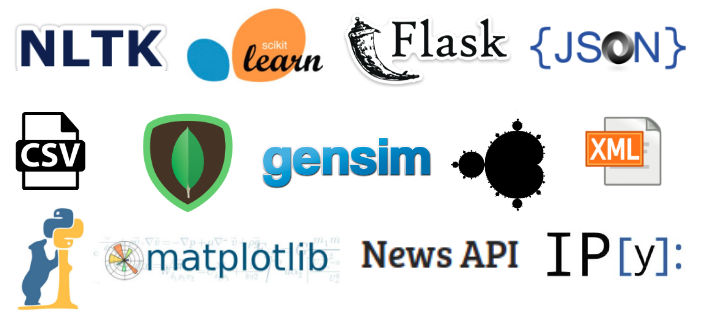
\includegraphics[height=150pt,width=320pt]{img/chapter4/tools/tools.png}
                    \caption{Logos de quelques librairies utilisées}
                    \label{}
            \end{figure}
            \begin{enumerate}[leftmargin=*]
                \item{\textbf{NLTK : }}
                "Natural Language Toolkit" est une librairie Python destinée au TALN. Elle fournit une suite de bibliothèques de traitement de texte pour la classification, tokenization, stemming, étiquetage, analyse et raisonnement sémantique, etc. \cite{nltk}.\\

                \item{\textbf{Scikit-Learn : }\label{scikit-learn}}
                Bibliothèque libre et Open source implémenté avec Python, dédiée à l'apprentissage automatique. Elle est conçue pour s'harmoniser avec d'autres bibliothèques Python (ou autres), notamment NumPy, SciPy, etc. \cite{scikit}.\\

                \item{\textbf{Numpy : }}
                "Numerical Python" fournit une interface pour stocker et effectuer des opérations sur les données. D'une certaine manière, les tableaux Numpy sont comme les listes en Python, mais Numpy permet de rendre les opérations beaucoup plus efficaces, surtout sur les tableaux de grande taille qui sont au cœur de l'écosystème de la Data Science \cite{numpy}.\\
                
                \item{\textbf{Gensim : }}
                Librairie Python gratuite conçue pour extraire automatiquement des sujets sémantiques à partir de documents. Les algorithmes de Gensim, tels que l'analyse sémantique latente, permettent de découvrir la structure sémantique des documents en examinant les schémas statistiques de cooccurrence des mots au sein d'un corpus de documents \cite{gensim}.\\

                \item{\textbf{Pandas : }}
                Fournit deux structures de données fondamentales, la "Série" et le "DataFrame". On peut voir ces structures comme une généralisation des tableaux et des matrices de Numpy. La différence entre les structures de Pandas et celles de Numpy c'est la définition explicites par l'utilisateur des indices et des index sur les objets (matrices) .\cite{pandas}\\

                \item{\textbf{Pickle : }}
                Module Python utilisé pour sérialiser et désérialiser les structures d'objets Python. La sérialisation (ou «pickling») fait référence au processus de conversion d'un objet en mémoire en un flux d'octets pouvant être stocké sur disque ou envoyé sur un réseau. Plus tard, ce flux de caractères peut être récupéré et désérialisé (ou «unpickling») en retour vers un objet Python \cite{pickle}.\\

                \item{\textbf{Matplotlib : }}
                "Mathematic Plot library" est une bibliothèque de traçage Python 2D qui produit des figures de qualité de publication dans une variété de formats papier et d'environnements interactifs entre plates-formes. Matplotlib peut être utilisé dans les scripts Python, les Shells Python et IPython, les notebook Jupyter, etc. \cite{matplotlib}.\\

                \item{\textbf{Newspaper : }}
                Librairie Python accessible gratuitement qui permet d'extraire le contenu, l'image, les auteurs et la date de publication d'un article de presse en utilisant le protocole HTTP.\\

                \item{\textbf{Newsapi : }}
                Web API qui permet d'obtenir des articles de presse de dernière minute et de rechercher des articles de plus de 30 000 sources et blogs. Elle fournit également la possibilité de sélectionner les sources, les pays, les catégories, etc.\\

                \item{\textbf{FeedParser : }}
                "Universal Feed Parser" est une librairie Python pour le téléchargement et l'analyse des flux syndiqués connu sous l'appellation \emph{flux RSS}. Cette librairie se distingue par sa facilité d'utilisation \cite{feedparser}.\\

                \item{\textbf{TextBlob : }}
                Toolbox Python pour le traitement des données textuelles. Elle fournit une API simple permettant de plonger dans des tâches courantes de TALN, telles que l'étiquetage, l'extraction de syntagmes nominaux, l'analyse des sentiments, la classification, la traduction automatique, etc. \cite{textblob}\\

                \item{\textbf{Farasa : }}
                L'équivalent arabe de "perspicacité", Farasa est une Toolbox de traitement de la langue naturel arabe développé au sein de l'institut \emph{Qatar Computing Research Institute}. Elle est composée de plusieurs modules : segmentation, étiquetage, etc. Farasa surpasse ou égalise les deux fameuses Toolbox pour l'arabe Stanford NLP et MADAMIRA \cite{farasa}.\\

                \item{\textbf{PyRouge : }}
                Interface Python pour le fameux module d'évaluation des résumés automatique ROUGE. Elle facilite l'utilisation de ROUGE avec la conversion des fichiers qui contiennent les résumés en un format interprétable par ROUGE et génère automatiquement les fichiers de configuration ROUGE \cite{pyrouge}.\\

                \item{\textbf{PyMongo}}
                Module de gestion du SGBD MongoDB sous le langage Python, il fournit une variété de commandes très intéressantes qui permettent de faciliter la manipulation d'une base de donnée NoSql \cite{pymongo}.\\
            \end{enumerate}

        \subsubsection{Formats de données}
            \begin{enumerate}[leftmargin=*]
                \item{\textbf{XML : }}
                "eXtensible Markup Language" est un langage informatique de balisage générique. Ces balises permettent de structurer de manière hiérarchisée et organisée les données d'un document.\\

                \item{\textbf{JSON : }}
                "JavaScript Object Notation" est un format adapté aux types de données du langage JavaScript. Au cours des dernières années, JSON est devenu l'un des premiers format d'échange et de stockage de données notamment pour le développement web \cite{jsonimpl}.\\
                
                \item{\textbf{CSV : }}
                "Comma-separated values" est un format informatique représentant des données tabulaires sous forme de valeurs séparées par des virgules. Le format de fichier CSV est utilisable par les applications de tableur KSpread, OpenOffice Calc, Microsoft Excel, etc. De nombreuses autres applications prennent en charge CSV pour importer ou exporter des données.\cite{csv}
            \end{enumerate}

        \subsubsection{Logiciels et éditeurs de textes}
            \begin{figure}[H]
                    \centering
                    
\includegraphics[height=80pt,width=250pt]{img/chapter4/tools/software.png}
                    \caption{Logos des logiciels utilisés}
                    \label{}
            \end{figure}
            \begin{enumerate}[leftmargin=*]
                \item{\textbf{PyCharm Community Edition : }}
                PyCharm est un éditeur de code pour le développement sous Python, il fournit la complétion de code intelligente, des inspections, la mise en évidence d'erreurs à la volée et des correctifs rapides, ainsi que des corrections de code automatisés et de riches fonctionnalités de navigation.\cite{pycharm} Le version \emph{Community Edition} que nous avons utilisé est gratuite et en libre accès.\\

                \item{\textbf{WebStorm : }}
                WebStorm est un éditeur de code pour le développement sous Javascript, il apporte une aide énorme au développeurs web et mobile. Il supporte tout les langages compilés au JavaScript, Node.js, HTML et CSS \cite{webstorm}. Nous avons pu obtenir une licence étudiant d'une année.\\

                \item{\textbf{Sublime Text : }}
                Éditeur de texte générique codé en C++ et Python, disponible sur Linux, Mac et Windows. Depuis la version 2.0, sortie le 26 juin 2012, l'éditeur prend en charge 44 langages de programmation majeurs, tandis que des plugins sont souvent disponibles pour les langages plus rares \cite{sublime}. Nous avons utilisé la version d’essai qui est en libre accès sur internet.\\

                \item{\textbf{Git : }}
                Système de gestion de versions décentralisé. C'est un logiciel libre créé par \emph{Linus Torvalds}, auteur du noyau Linux, et distribué selon les termes de la licence publique générale (GPL). En 2016, il s’agit du logiciel de gestion de versions le plus populaire qui est utilisé par plus de douze millions de personnes \cite{git}.
            \end{enumerate}



\section{Recommandation}
\subsection{Approche probabilité de sélection}  
Afin d'implémenter cette approche et tenter de générer une collection de profils utilisateurs, nous avons essayer d'utiliser des datasets destinés au articles de presse. Ci-dessous, une description des datasets utilisés.

\subsubsection{SmartMedia Adressa News Dataset}
Le dataset Adressa est un ensemble de données d'actualité comprenant des articles de presse (en norvégien) en lien avec des utilisateurs anonymes. Cet ensemble de données est publié avec la collaboration de l'Université norvégienne des sciences et technologies (NTNU) et Adressavisen (journal local à Trondheim, Norvège) dans le cadre du projet RecTech sur la technologie de recommandation.\cite{refnorvege}

\subsubsection{Structure du dataset}


Exemple :


\subsubsection{Statistiques sur le dataset}


\subsubsection{Inconvénients de l'utilisation de \textquotedbl SmartMedia Adressa News Dataset\textquotedbl}

Le dataset décrit dans cette partie traite les articles de presse en langage nowégien, c'est a dire que les catégories des articles sont en norwégien et le contenu des articles aussi. Ce qui nous a amené a abandonné ce dataset.
  
\subsubsection{Le dataset \textquotedbl YOW \textquotedbl}
Afin de concevoir une base de données de profils utilisateurs, nous avons solliciter \emph{Google News}, \emph{Bing News} et \emph{Yahoo Webscope} mais sans aucune réponse de la part de ces entreprises. 

Mais au final, nous avons pu obtenir le dataset \emph{YOW} qui est le seul dataset d'interactions des profils avec des articles de presse. 

\emph{Yow} été collecté à l'Université \emph{Carnegie Mellon} pour le \emph{Yow-now} le système de filtrage des articles de presse \cite{carnegieYOW}.

Le dataset YOW est composé de plusieurs attribut, des informations sur les interactions de 22 utilisateurs avec des articles de presse de différentes catégories. Les instances du dataset sont très bien adapté au filtrage collaboratif. Comme il n'y a pas d'information sur le contenu des articles de presse, le filtrage basé sur le contenu n'est pas possible. 

\subsubsection{Structure du dataset}
Chaque instance du dataset YOW est composé de 23 attribut propre à l'utilisateur et à l'article de presse. Ci-après les attributs les plus importants pour notre système de recommandations :  
\begin{lstlisting}[style=code] 
{
'user_id': '19', 
'document_id': '27010084'
'timestamp': '2004-04-23T15:38:25Z'
'timeonpage': '63s', #temps de lecture
'classes': [
'space', 'international', 'iraq', 
],
...
},
\end{lstlisting}

\subsubsection{Statistiques sur le dataset}
Yow-now est un système de filtrage d'informations qui recommande des articles de presse aux utilisateurs à partir de divers flux RSS. Les données sont recueillies par une étude d'un mois qui comprend environ 25 personnes et plus de 7000 entrées de commentaires de tous les utilisateurs. Au total 383 articles évalués par chaque utilisateur. 

Le dataset comporte également des évaluations implicite et explicite sur les recommandations. Le profilage explicite est sous forme de note de 1 à 5, quant à l'implicite est établi selon les interactions de l'utilisateur (souris, clavier et activités de défilement).


\subsubsection{Pré-traitement des données}
Chaque instance du dataset \emph{YOW} est une interaction de l'utilisateur U avec un article A.

L'interaction peut avoir plusieurs valeurs pour l'attribut \emph{Classe} (catégorie dans notre cas). "Classe" peut prendre des noms de catégories et des mots-clés de l'article, par exemple :
\begin{itemize}
    \item Noms de catégories : world, science, entertainment, space, business, food, etc.
    \item Mots-clés :Iraq, Amazon, Malaysia, Oil, Japan, etc.\\ 
\end{itemize}
Pour adapter ces données à notre modèle de catégorisation d'article nous avons effectué des pré-traitement sur chaque instance du dataset. Nous avons annoter le dataset manuellement dans le but de convertir les noms de catégories et les mots-clés en catégories présente dans notre système (7 pour l'Anglais et 6 pour l'Arabe), par exemple :
\begin{itemize}
    \item Avant : nuclear weapons, international, middle east, business, John Kerry, accident, tradegy, space, science.
    \item Après : 
    \begin{itemize}
        \item {nuclear weapons, international, middle east} : World
        \item {John Kerry} : US
        \item {space, science} : Science \& Technology
        \item {accident, tradegy} : Society
        \item {business} : Business\\
    \end{itemize}    
\end{itemize}
De plus, le dataset a été classé dans l'ordre croissant de l'attribut "Timestamp", la date et l'horaire de l'interaction, dans le but de récupérer l'historique et le changement des centres d’intérêts de chaque utilisateur. 

À chaque nouvelle interaction le vecteur de probabilité de sélection des catégories d'articles se mets à jour en fonction de l'article visité. 

La mise à jour consiste en l'augmentation de la probabilité de sélection de la catégorie de l'article choisie et la diminution des autres catégories (s'il y-en a). 

L'exemple suivant montre le processus de mise à jour :
\begin{itemize}[label={}]
    \item $P = {'news': 0.0581,'sport': 0.717, 'sci\_tech': 0.149}$\\
\end{itemize}

L'utilisateur X a cliqué et lu un article de la catégorie \emph{Sport}, le vecteur de probabilité de sélection va se mettre à jour en fonction de cette dernière interaction (détails dans \ref{proba-select}).
\begin{itemize}[label={}]
    \item $P[sport] = (1-{\alpha}) * {P[sport]} + {\alpha}$
    \item $P[sport] = (1-{0.1}) * {P[sport]} + {0.1}$
    \item $P[sport] = (1-{0.1}) * {0.717} + {0.1}$
    \item $P[sport] = 0.745$
\end{itemize}

Quant aux autres catégories du vecteurs de sélection :
\begin{itemize}[label={}]
    \item $P[news] = (1-{\alpha}) * {P[news]} $
    \item $P[news] = (1-{0.1}) * {P[news]} $
    \item $P[news] = (1-{0.1}) * {0.0581} $
    \item $P[news] = 0.0523$
    \item 
    \item $P[sci\_tech] = (1-{\alpha}) * {P[sci\_tech]} $
    \item $P[sci\_tech] = (1-{0.1}) * {P[sci\_tech]} $
    \item $P[sci\_tech] = (1-{0.1}) * {0.1499} $
    \item $P[sci\_tech] = 0.135$
\end{itemize}
Après cette interaction, le vecteur de probabilité de sélection devient :
\begin{itemize}[label={}]
    \item $P = {'news': 0.0523, 'sport': 0.745, 'sci_tech': 0.135}$\\
\end{itemize}
Pour un nouvel utilisateur, le même traitement est appliqué, le vecteur de probabilité de sélection se remplie petit à petit en fonction des interaction qui vont être mise à jour de la même façon.

\subsubsection{Utilisateur non identifier}
Dans le cas où l'utilisateur n'est pas connecté, donc il n’y a pas de vecteur de probabilité de sélection, la recommandation est basée sur la similarité entre articles.

Si l'utilisateur U a lu l'article A1, les articles A2, A3, ..., An similaires à A1, seront recommandés. La similarité entre article est calculé à partir du contenu, le texte sera convertit en TF-IDF et les articles les plus proches en calculant la similarité du Cosinus seront considérés comme article qui parle du même sujet ou de la même catégorie.

\begin{itemize}[leftmargin=*]
    \item Exemple :\\ 
    A1 = "Real Madrid 3-1 Liverpool: Jurgen Klopp says Reds wanted everything and got minus something"\\
    Articles similaires à A1 = \{\\
    'Gareth Bale on his Champions League final goal for Real Madrid': 0.26435,\\
    'Real Madrid 3-1 Liverpool: ‘Flawed Karius pays for lack of focus’': 0.21839,\\
    'Columbus Crew: Two US cities fight over one football team': 0.073586
    \}
\end{itemize} 

\section{Catégorisation}
    Le deuxième module sur lequel nous avons travailler, c'est la catégorisation d'articles de presse. Nous avons expérimenter plusieurs techniques proposées dans la littérature. Nous présentons ci-après chaque approche, ses résultats, ses points forts et ses faiblesses.
    \subsection{Approches expérimentées\label{approches}}
        Toutes les approches utilisées sont basées sur l'apprentissage automatique, supervisé et non supervisé. 
        \subsubsection{Basées sur l'Apprentissage Non Supervisé}
            \begin{itemize}
                \item{LDA (Latent Dirichlet Allocation) : }
            \end{itemize}

        \subsubsection{Basées sur l'Apprentissage Supervisé}
            \begin{table}[H]
                    \begin{center}
                        \begin{tabular}{|c|c|c|c|c}
                            \hline
                            \textbf{Modèle} & \textbf{Précision} & \textbf{Rappel} & \textbf{F-mesure} \\
                            \hline
                            Naïve de Bayes & 0.89 & 0.87 & 0.88 \\
                            Arbre de décision & 0.82 & 0.84 & 0.83 \\
                            \textbf{Descente de Gradient Stochastique} & \textbf{0.94} & \textbf{0.94} & \textbf{0.94} \\
                            SVM & 0.91 & 0.89 & 0.90 \\
                            \hline
                        \end{tabular}
                    \end{center}
                    \caption{Résultats comparatifs des modèles de catégorisation pour l'arabe}
                    \label{modele-categ}
                \end{table}
                
    \subsection{Corpus et dataset}
        Comme tout problème de classification, la catégorisation d'articles de presse nécessite de très grandes masses de données. C'est pour cela que nous avons consacrer une bonne période du projet à la récolte des corpus et la préparation des datasets.     
        \subsubsection{Quelques chiffres et statistique}
            \begin{itemize}
                \item{\textbf{Anglais : }}
                 Le dataset baptisé "News" a été récolté par le Laboratoire Informatique de \emph{l'Université de Pise} \cite{pise}, il regroupes des articles de 3 sources différentes : \emph{The New York Times}, \emph{Reuters} et \emph{USA Today}. le Tableau \ref{news-categ} présente en détails le nombre d'articles de chaque catégorie.
                \begin{table}[H]
                    \begin{center}
                        \begin{tabular}{|C{5cm}|C{5cm}|}
                            \hline
                            \textbf{Catégorie} &  \textbf{Nombre d'articles} \\
                            \hline
                            Business & 5366 \\                            
                            Entertainment & 3286 \\
                            Health & 1851 \\
                            Science \& Technology & 2872 \\
                            Sport & 8189 \\
                            US & 4783 \\
                            World & 6255 \\
                            \textbf{Totale} &  \textbf{32602} \\
                            \hline
                        \end{tabular}
                    \end{center}
                    \caption{Nombres d'articles de chaque catégorie du corpus "News"}
                    \label{news-categ}
                \end{table}
                \item{\textbf{Arabe : }}
                Le corpus TALAA\footnote{Traitement Automatique du Langage et Apprentissage Automatique, l'équipe de recherche du Laboratoire de Recherche en Intelligence Artificielle du département informatique de l'USTHB} pour la catégorisation d'articles de presse est une grande collection d'articles publiés entre 2010 et 2014 dans différentes revue de presse Arabe sur internet. Il contient plus de 14 millions de mots de 582000 types différents. Le corpus contient 8 catégories, mais nous avons choisi de travailler sur 6 catégories plus générales comme on peut le constater dans le tableau suivant \ref{talaa-categ} \cite{talaa}. 
                \begin{table}[H]
                    \begin{center}
                        \begin{tabular}{|c|c|}
                            \hline
                            \textbf{Catégorie} &  \textbf{Nombre d'articles} \\
                            \hline
                            \begin{arab}الجزائر\end{arab} & 6603 \\
                            \begin{arab}الثقافة\end{arab} & 3311 \\
                            \begin{arab}الدين\end{arab} & 2568 \\
                            \begin{arab}المجتمع\end{arab} & 7714 \\
                            \begin{arab}الرياضة\end{arab} & 8104 \\
                            \begin{arab}العالم\end{arab} & 4380 \\
                            \textbf{Totale} & \textbf{32680} \\
                            \hline
                        \end{tabular}
                    \end{center}
                    \caption{Nombres d'articles des 6 catégories choisies du corpus "TALAA"}
                    \label{talaa-categ}
                \end{table}
            \end{itemize}
        \subsubsection{Pré-traitement et structure des datasets}
            Les deux corpus utilisés dans les deux langues étaient sous le format brute, ce qui nécessitaient une restructuration et un pré-traitement afin de permettre leur exploitation.  

            Plusieurs opérations de pré-traitements ont été effectuées. Ci-après les étapes suivies :
            \begin{enumerate}
                \item{\textbf{Segmentation (Tokenization) et suppression des mots vides :} } Pour l'Anglais nous avons utiliser le Tokenizer natif de NLTK, et FARASA Toolbox pour la langue Arabe.\\  
                
                \item{\textbf{Racinisation (Stemming) :} } 
                La librairie Snowball Stemmer de NLTK a été utilisé pour l'Anglais, quant à l'Arabe c'est toujours la Toolbox FARASA.\\

                \item{\textbf{N-grammes :} }
                 L'algorithme natif de NLTK a été utilisé pour les deux langues (Anglais et Arabe).\\ 
                
                \item{\textbf{Extraction des caractéristiques :} }
                Les librairies Countvectorizer et tfidfvectorizer de scikit-learn ont été utilisés dans l'éxtraction des caractéristiques pour l'anglais et l'arabe.\\
            \end{enumerate}

            
    \subsection{Modèles finaux}
        Après expérimentation des techniques citées dans \ref{approches}, voici les modèles finaux de la catégorisation d'articles de presse implémentés en Python en utilisant la librairie Scikit-learn \ref{scikit-learn} :
        \begin{itemize}
            \item{\textbf{Anglais :} }le modèle le plus performant est obtenu en utilisant l'algorithme SVM avec 80\% de données pour l'apprentissage et le 20\% restant pour les tests sur un total de 32602 articles de 7 catégories différentes.\\

            \item{\textbf{Arabe :} }l'algorithme de la Descente de Gradient Stochastique nous a donné les meilleurs résultats en utilisant 32680 articles, avec 75\% de données pour l'apprentissage et le reste pour les tests. 
        \end{itemize}
    \subsection{Résultats et évaluation}
        \subsubsection{Résultats}
        \begin{itemize}
            \item{\textbf{Anglais :}}
            \begin{itemize}
                \item{Accuracy : 0.987}
                \item{Précision : 0.988}
                \item{Rappel : 0.982}
                \item{F-mesure : 0.985}
            \end{itemize}
            \begin{table}[H]
                    \begin{center}
                        \begin{tabular}{|c|C{2cm}|C{2cm}|C{2cm}|C{2cm}|}
                            \hline
                            \textbf{Catégorie} &  \textbf{Précision} &  \textbf{Rappel} &  \textbf{F-mesure} &  \textbf{Support} \\
                            \hline
                            Business & 0.98 & 0.96 & 0.97 & 1046 \\
                            Entertainment & 0.99 & 0.99 & 0.99 & 651 \\
                            Health & 0.97 & 1.00 & 0.99 & 388 \\
                            Science \& Technology & 0.94 & 1.00 & 0.97 & 546 \\
                            Sport & 1.00 & 1.00 & 1.00 & 1635 \\
                            US & 0.99 & 0.98 & 0.99 & 993 \\
                            World & 1.00 & 0.99 & 0.99 & 1262 \\                          
                            \textbf{Moyenne/Totale} & \textbf{0.99} & \textbf{0.98} & \textbf{0.99} & \textbf{6521} \\
                            \hline
                        \end{tabular}
                    \end{center}
                    \caption{Résultat global et pour chaque catégorie de la catégorisation pour l'Anglais}
            \end{table}
            \item{\textbf{Arabe :}}
            \begin{itemize}
                \item{Accuracy : 0.936}
                \item{Précision : 0.94}
                \item{Rappel : 0.94}
                \item{F-mesure : 0.94}
            \end{itemize}
            \begin{table}[H]
                    \begin{center}
                        \begin{tabular}{|c|C{2cm}|C{2cm}|C{2cm}|C{2cm}|}
                            \hline
                            \textbf{Catégorie} &  \textbf{Précision} &  \textbf{Rappel} &  \textbf{F-mesure} &  \textbf{Support} \\
                            \hline
                            \begin{arab}الجزائر\end{arab} & 0.93 & 0.88 & 0.91 & 664 \\
                            \begin{arab}الثقافة\end{arab} & 0.91 & 0.86 & 0.88 & 509 \\
                            \begin{arab}الدين\end{arab} & 0.94 & 0.92 & 0.93 & 860 \\
                            \begin{arab}المجتمع\end{arab} & 0.91 & 0.94 & 0.92 & 1541 \\
                            \begin{arab}الرياضة\end{arab} & 0.99 & 0.99 & 0.99 & 1620 \\
                            \begin{arab}العالم\end{arab} & 0.92 & 0.94 & 0.93 & 1316 \\                      
                            \textbf{Moyenne/Totale} & \textbf{0.94} & \textbf{0.94} & \textbf{0.94} & \textbf{6510} \\
                            \hline
                        \end{tabular}
                    \end{center}
                    \caption{Résultat global et pour chaque catégorie de la catégorisation pour l'Arabe}
                \end{table}
        \end{itemize}

        \subsubsection{Évaluations}
        \begin{itemize}[leftmargin=*]
            \item{\textbf{Anglais :} }\\
                Le \autoref{confusion-anglais} présente la matrice de confusion du module de catégorisation d'articles de presse pour l'Anglais. On peut constater qu'il y-a très peu de confusion entre les différentes catégories, à part quelques articles comme les 31 articles qui ont été prédits comme \emph{Science \& Technology} alors qu'ils appartiennent à la catégorie \emph{Business}, cela est dû au contenu de ces articles qui doivent parlés de business dans le domaine de la science et technologie. 
                \begin{table}[H]
                    \begin{center}
                        \begin{tabular}{|c|c|c|c|c|c|c|c|}
                            \cline{2-8}
                            \multicolumn{1}{c|}{} & \textbf{Sport} &  \textbf{World} &  \textbf{News} &  \textbf{Business} &  \textbf{Health} & \textbf{Entert.\footnote{Entertainment}} &  \textbf{Sci-Tech} \\
                            \hline
                            \textbf{Sport} & 1635 & 0 & 0 & 0 & 0 & 0 & 0 \\
                            \textbf{World}  & 0 & 1249 & 0 & 9 & 2 & 1 & 1 \\
                            \textbf{News}  & 0 & 0 & 974 & 11 & 3 & 3 & 2 \\
                            \textbf{Business}  & 0 & 5 & 4 & 1003 & 3 & 0 & 31 \\
                            \textbf{Health}  & 0 & 0 & 0 & 0 & 388 & 0 & 0 \\
                            \textbf{Entert.}  & 0 & 0 & 0 & 1 & 3 & 646 & 1 \\
                            \textbf{Sci-Tech}  & 0 & 0 & 1 & 0 & 0 & 1 & 544 \\
                            \hline
                        \end{tabular}
                    \end{center}
                    \caption{Matrice de confusion du modèle de la catégorisation d'articles Anglais}
                    \label{confusion-anglais}
                \end{table}
                % \item{Courbe ROC : }
                % \begin{figure}[H]
                %     \centering
                %     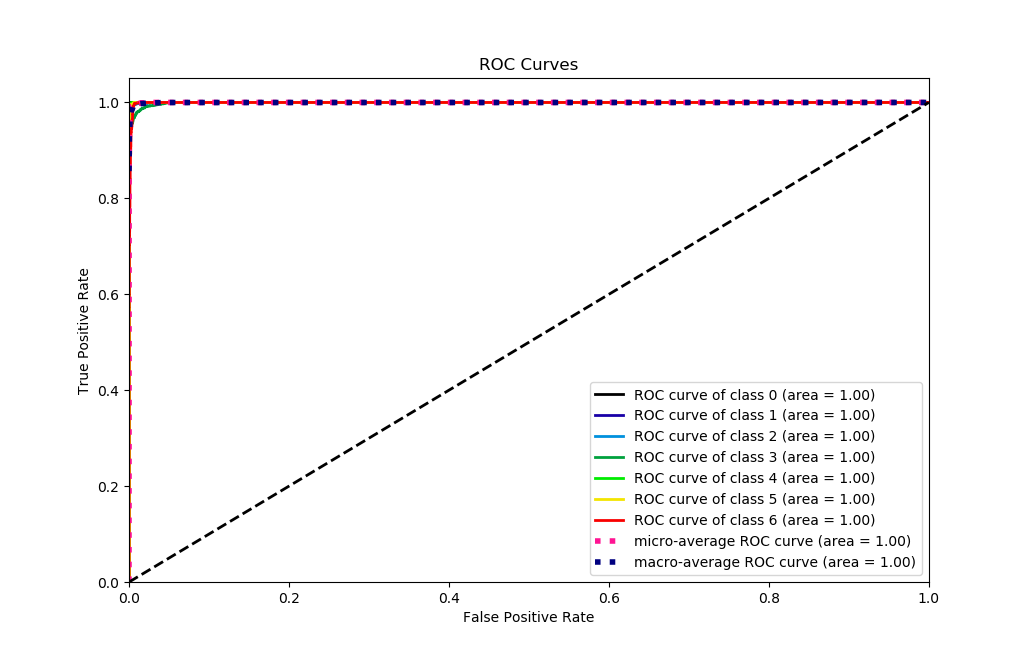
\includegraphics[height=320pt,width=330pt]{img/chapter4/rocEN.png}
                %     \caption{}
                %     \label{}
                % \end{figure}
            \item{\textbf{Arabe :} }\\
                Tout comme l'Anglais le modèle développé pour l'Arabe, a montré une capacité de prédiction très élevée. Comme on peut le voire dans le \autoref{confusion-arabe}, la confusion entre les catégories est très faible à part quelques articles des catégories proches en terme de contenu. 
                \begin{table}[H]
                    \begin{center}
                        \begin{tabular}{|c|c|c|c|c|c|c|}
                            % \cline{2-7}
                            % \hline
                            % \multicolumn{1}{c|}{} & \multicolumn{6}{|c|}{Predicted} \\
                            % \hline
                            \cline{2-7}
                            \multicolumn{1}{c|}{} & \textbf{\begin{arab}العالم\end{arab}} &  \textbf{\begin{arab}الرياضة\end{arab}} &  \textbf{\begin{arab}الجزائر\end{arab}} &  \textbf{\begin{arab}المجتمع\end{arab}} &  \textbf{\begin{arab}الدين\end{arab}} &  \textbf{\begin{arab}الثقافة\end{arab}} \\
                            \hline
                            \textbf{\begin{arab}العالم\end{arab}} & 1232  &  1  & 11 &  51  & 18  &  3 \\
                            \textbf{\begin{arab}الرياضة\end{arab}}  & 1 & 1609  &  1  &  6  &  3 &   0 \\
                            \textbf{\begin{arab}الجزائر\end{arab}}  & 28  &  2 & 587 &  21  &  9  & 17 \\
                            \textbf{\begin{arab}المجتمع\end{arab}}  & 43  & 11 &  17& 1447 &  12 &  11 \\
                            \textbf{\begin{arab}الدين\end{arab}}  & 36  &  0  &  6 &  18 & 788 &  12 \\
                            \textbf{\begin{arab}الثقافة\end{arab}}  & 3  &  0 &   8 & 53  &  9 & 436 \\
                            \hline
                        \end{tabular}
                    \end{center}
                    \caption{Matrice de confusion du modèle de la catégorisation d'articles Arabe}
                    \label{confusion-arabe}
                \end{table}

                % \item{Courbe ROC : }
                % \begin{figure}[H]
                %     \centering
                %     \includegraphics[height=320pt,width=330pt]{img/chapter4/ux/1.png}
                %     \caption{}
                %     \label{}
                % \end{figure}
        \end{itemize}

\section{Résumé automatique}
    La deuxième partie de la phase de réalisation est consacrée au résumé automatique. Nous avons expérimentés plusieurs techniques et méthodes que nous allons voire en détails dans cette section. 
    \subsection{Approches expérimentées}
        \subsubsection{Résumé extractif par Apprentissage Supervisé}
            Nous avons commencé par une approche basée sur l'apprentissage automatique supervisé, ce qui nécessitait des corpus d'articles avec leur résumés types.
            \begin{itemize}
                 \item{\textbf{Contribution à la récolte de données : "Sumrized" et "Mou3in"}}\\
                Face au manque flagrant des corpus (gratuits) pour le résumé automatique, nous avons développer une plate-forme contributive sur le web baptisée \textbf{Sumrized.com} pour la récolte des textes et des résumés en trois langues Arabe, Anglais et Français. 

                Chaque texte et son résumé sont vérifier manuellement par un expert qui peut consulter et valider les contributions à partir d'un Dashboard dédié à cet effet. L'interface principale de la plate-forme, qui est en ligne depuis Février 2018, est présentée dans la figure \ref{sumrized-ui}. 

                \begin{figure}[H]
                    \centering
                    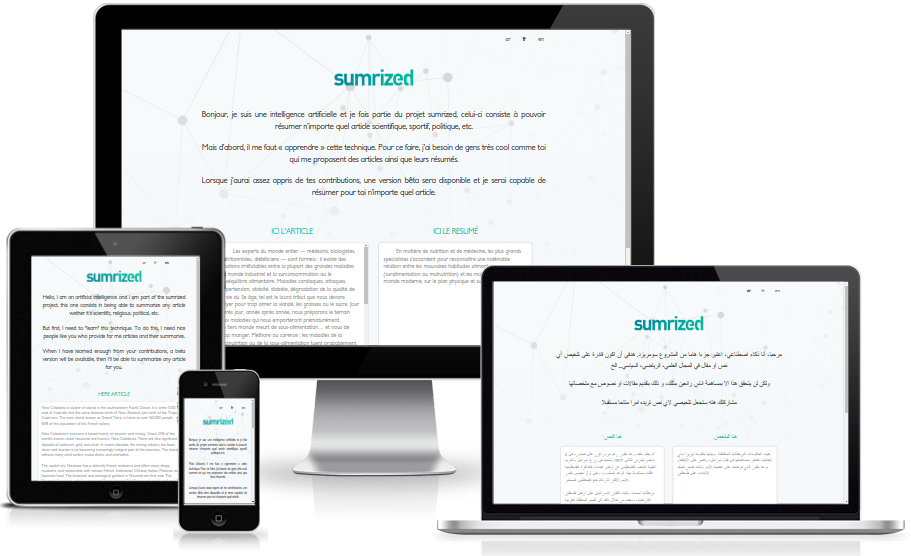
\includegraphics[height=180pt,width=320pt]{img/chapter4/sumrized/responsive.png}
                    \caption{La plate-forme Sumrized sur les différents supports}
                    \label{sumrized-ui}
                \end{figure} 

                Nous avons également développé une application de bureau, appelée \textbf{Mou3in}, afin de faciliter l'annotation des textes, elle offre à son utilisateur la possibilité d'attribuer une étiquette à chaque phrase selon son jugement (à supprimer ou à laisser). La figure \ref{mou3in} présente l'espace de travail sur l'application "Mou3in" :
                \begin{figure}[H]
                    \centering
                    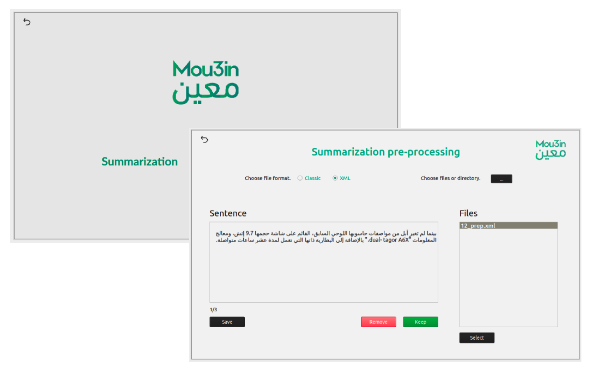
\includegraphics[height=230pt,width=370pt]{img/chapter4/mou3in/mou3in.png}
                    \caption{Interface utilisateur de "Mou3in"}
                    \label{mou3in}
                \end{figure}

                \item{\textbf{Pré-traitement et structure du dataset}}\\
                Tout les articles du dataset sont sous le format XML, chaque article a son propre identifiant et divisé en paquets de phrases selon l'opération effectuée. Ci-après la figure \ref{xml-structure} qui montre un exemple du dataset : 
                \begin{figure}[H]
                    \centering
                    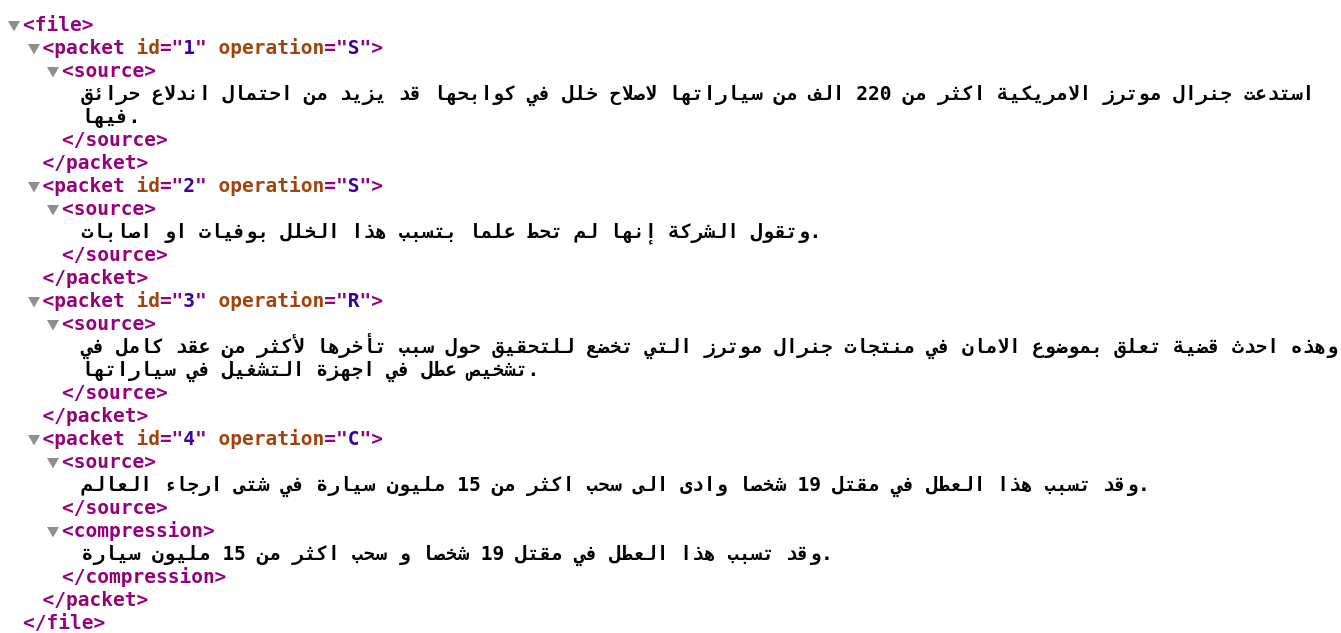
\includegraphics[height=220pt,width=430pt]{img/chapter4/xml.png}
                    \caption{Structure d'un article du dataset}
                    \label{xml-structure}
                \end{figure}
                L'approche basée sur l'apprentissage automatique demandait un très grand nombre d'articles résumés, ce qui nous a poussé à l'abandonner.
            \end{itemize}
        \subsubsection{Résumé extractif par Machine de Boltzman}
            L'approche proposée dans \cite{boltzman} utilise un modèle d'apprentissage profond afin de prédire les phrases les plus importantes dans un texte donnée en utilisant 9 caractéristiques sur chaque phrase. Elle consiste en trois grande phases: l'extraction des caractéristiques, la conversion en valeurs numériques et la génération du résumé à partir des scores de chaque phrase. 

            \begin{itemize}[leftmargin=*]
                \item{\textbf{Pré-traitement et structure du dataset}}\\
                Cette méthode, contrairement aux autres, est appliquée sur un seul document, on a pas besoin de plusieurs documents. La texte est segmenté en phrase, chaque phrase est divisé en mots et les caractéristiques citées là-dessus sont calculées.\\

                La matrice qui représentent le texte est injectée dans une Machine de Boltzman\footnote{Type de réseau de neurones artificiels pour l'apprentissage non supervisé} afin de calculé les score des phrases. Les résultats sont triés dans l'ordre décroissant des scores et le résumé est établi selon ces derniers.\\

                \item{\textbf{Résultats et critiques}}\\
                L'évaluation de ce modèle est effectuée en utilisant le \emph{Gold Standard}\footnote{Dataset de référence construit par des experts linguistes, utilisé pour l'évaluation des résultats} Duc2004 qui est un dataset qui contient 50 articles de presse de différentes catégories et 4 à 5 résumés de référence pour chaque article.

                Nous avons obtenu les résultats présentés dans le \autoref{result-boltzman} en utilisant ROUGE (les métriques d'évaluations, ROUGE notamment, sont définies dans la \autoref{metrique-eval}) : 
                \begin{table}[H]
                    \begin{center}
                        \begin{tabular}{|c|C{1.2cm}|C{1.2cm}|C{1.2cm}|C{1.2cm}|C{1.2cm}|C{1.2cm}|C{1.2cm}|C{1.2cm}|}
                            \cline{2-9}
                            \multicolumn{1}{c|}{} & \textbf{R-1} &  \textbf{R-2} &  \textbf{R-3} &  \textbf{R-4} &  \textbf{R-L} &  \textbf{R-W} &  \textbf{R-S} &  \textbf{R-SU} \\
                            \hline
                            \textbf{Rappel} & 0.4172 & 0.0615 & 0.0129 & 0.0042 & 0.3239 & 0.1089 & 0.1693 & 0.1739 \\
                            \textbf{Précision} & 0.1982 & 0.0264 & 0.0054 & 0.0016 & 0.1525 & 0.0919 & 0.0385 & 0.0402 \\
                            \textbf{F-mesure} & 0.2549 & 0.0346 & 0.0071 & 0.0022 & 0.1963 & 0.0934 & 0.0556 & 0.0578 \\
                            \hline
                        \end{tabular}
                    \end{center}
                    \caption{Résultats du résumeur extractif basé sur la Machine de Boltzman}
                    \label{result-boltzman}
                \end{table}
                En effet, ces résultats sont très proches des résumeurs de l'état de l'art, mais le modèle que nous avons utilisé est pré-entraîné sur un type de données totalement différent (des images), ce qui nous a amené à laisser tomber cette approche.   
            \end{itemize}

        \subsubsection{Résumé extractif par Plongement de mots\ref{plongement}}
        L'approche proposée par l'équipe de recherche du département informatique de l'Université de Bari en Italie \cite{bari}, est basée sur la similarité textuelle entre la phrase centroïde et les autres phrases du texte en utilisant les plongements de mots (Word embeddings). La conception et l'algorithme de réalisation sont détaillés dans \ref{plongement}       

    \subsection{Résultats et évaluation}
        \subsubsection{Métrique d'évaluation : ROUGE\label{metrique-eval}}
        ROUGE est l'acronyme de "Recall-Oriented Understudy for Gisting Evaluation". Il s'agit essentiellement d'un ensemble de métriques permettant d'évaluer le résumé automatique de textes ainsi que la traduction automatique. Il fonctionne en comparant un résumé produit automatiquement ou une traduction à un ensemble de résumés de référence (généralement produits par des humains). \cite{rouge0}
    
        \subsubsection{Types des métriques de ROUGE\label{type-rouge}}
        \begin{itemize}
            \item{ROUGE-1, 2, 3 et 4 : font référence au chevauchement des uni-grammes, bi-grammes, tri-grammes et quadri-grammes, respectivement, entre le système et les résumés de référence \cite{rouge1}.}\\
            \item{ROUGE-L, W : basés sur la plus longue sous-séquence commune (LCS) \cite{rouge2}.}\\
            \item{ROUGE-S : basé sur les cooccurrences des paires de mots dans l'ordre des phrases \cite{rouge2}.}\\
            \item{ROUGE-SU : en plus des paires de mots, il utilise aussi la cooccurrence mot unique toujours dans l'ordre des phrases.}
        \end{itemize}
    
        \subsubsection{Résultats du modèle de résumé automatique final}
        \begin{table}[H]
            \begin{center}
                \begin{tabular}{|c|C{1.2cm}|C{1.2cm}|C{1.2cm}|C{1.2cm}|C{1.2cm}|C{1.2cm}|C{1.2cm}|C{1.2cm}|}
                    \cline{2-9}
                    \multicolumn{1}{c|}{} & \textbf{R-1} &  \textbf{R-2} &  \textbf{R-3} &  \textbf{R-4} &  \textbf{R-L} &  \textbf{R-W} &  \textbf{R-S} &  \textbf{R-SU} \\
                    \hline
                    \textbf{Rappel} & 0.5631 & 0.1226 & 0.0346 & 0.0139 & 0.5111 & 0.1729 & 0.2981 & 0.3029 \\
                    \textbf{Précision} & 0.1662 & 0.0361 & 0.0105 & 0.0042 & 0.1503 & 0.0912 & 0.0281 & 0.0289 \\
                    \textbf{F-mesure} & 0.2485 & 0.0541 & 0.0157 & 0.0063 & 0.2245 & 0.1145 & 0.0488 & 0.0503 \\
                    \hline
                \end{tabular}
             \end{center}
            \caption{Résultats du résumeur extractif basé sur le plongement de mots}
            \label{result-boltzman}
        \end{table}

\section{Traduction Automatique}
Comme il a été décrit dans le chapitre précédent, la traduction sera intégrée directement à l'application finale afin d'offrir une fonctionnalité de traduction en plus de celle du résumé et la catégorisation. A cet effet, nous avons utilisé la bibliothèque TextBlob qui offre une traduction multilingues d'un article ou d'un résumé.
    \subsection{Exemple de traduction automatique}
    \begin{itemize}
        \item Anglais :\\ 
        \textquotedbl The Interior Ministers of Spain and Algeria signed an agreement this week to form a joint team of investigation with the goals of fighting “illegal migration” and “preventing Islamist terrorism.” The agreement comes after recent crackdowns by the Algerian authorities during the first months of 2018 have reduced the number of undocumented Algerian migrants arriving in Spain, a reduction that was praised by the Spanish Interior Minister Juan Ignacio Zoido at their meeting in Madrid.\textquotedbl \\
        
        \item Arabe :\\
        \textquotedbl وقع وزيرا الداخلية الإسباني والجزائري اتفاقا هذا الأسبوع لتشكيل فريق مشترك من التحقيق بهدف محاربة "الهجرة غير الشرعية" و "منع الإرهاب الإسلامي". ويأتي هذا الاتفاق بعد الإجراءات القمعية الأخيرة التي قامت بها السلطات الجزائرية خلال الأشهر الأولى من خفّض عام 2018 عدد المهاجرين الجزائريين غير الشرعيين الذين وصلوا إلى إسبانيا ، وهو تخفيض أشاد به وزير الداخلية الإسباني خوان إغناسيو زويدو في اجتماعهم في مدريد. \textquotedbl
    
        \item Français :\\
        \textquotedbl Les ministres de l'Intérieur d'Espagne et d'Algérie ont signé cette semaine un accord pour former une équipe conjointe d'enquête ayant pour objectif de lutter contre les "migrations clandestines" et "la prévention du terrorisme islamiste." L'accord intervient après les récentes mesures de répression des autorités algériennes. 2018 ont réduit le nombre de migrants algériens sans papiers arrivant en Espagne, une réduction qui a été saluée par le ministre espagnol de l'Intérieur Juan Ignacio Zoido lors de leur réunion à Madrid.\textquotedbl \\

   \end{itemize}